\documentclass{beamer}

\usepackage{pgfplots}
\usepackage{pgfplotstable}
\usepackage{tikz}
\usepackage{xcolor}

\usepgfplotslibrary{fillbetween}
\usepgfplotslibrary{groupplots}

\usetikzlibrary{arrows}
\usetikzlibrary{arrows.meta}
\usetikzlibrary{calc}
\usetikzlibrary{positioning}

\usetheme{UiO}

\definecolor{ds002424}{HTML}{FF0028}
\definecolor{HBN}{HTML}{FF000E}
\definecolor{ABCD}{HTML}{FF0C00}
\definecolor{QTAB}{HTML}{FF2D00}
\definecolor{PING}{HTML}{FF4800}
\definecolor{ADHD200}{HTML}{FF6800}
\definecolor{PNC}{HTML}{FF8300}
\definecolor{ABIDE II}{HTML}{FFA400}
\definecolor{ds000119}{HTML}{FFBF00}\definecolor{ADHD}{HTML}{FF0028}
\definecolor{ANX}{HTML}{FF6E00}
\definecolor{ASD}{HTML}{F8FF00}
\definecolor{BIP}{HTML}{5BFF00}
\definecolor{DEM}{HTML}{00FF3B}
\definecolor{MCI}{HTML}{00FFD7}
\definecolor{MDD}{HTML}{008FFF}
\definecolor{MS}{HTML}{0E00FF}
\definecolor{PARK}{HTML}{A600FF}
\definecolor{SCZ}{HTML}{FF00BF}
\definecolor{HC}{HTML}{7F7F7F}
\definecolor{CoRR}{HTML}{15FF00}
\definecolor{HCP}{HTML}{00FF05}
\definecolor{FCON1000}{HTML}{00FF20}
\definecolor{ds000171}{HTML}{00FF40}
\definecolor{TOP}{HTML}{00FF5B}
\definecolor{SCZ-Z}{HTML}{00FF7B}
\definecolor{NIMH}{HTML}{00FF96}
\definecolor{NKI-RS}{HTML}{00FFB6}
\definecolor{MPI-LEMON}{HTML}{00FFD1}
\definecolor{ds003592}{HTML}{00FFF1}
\definecolor{ds004302}{HTML}{00F1FF}
\definecolor{ds000222}{HTML}{00D5FF}
\definecolor{SALD}{HTML}{00B5FF}
\definecolor{IXI}{HTML}{009AFF}
\definecolor{DLBS}{HTML}{0079FF}
\definecolor{Cam-CAN}{HTML}{005EFF}
\definecolor{StrokeMRI}{HTML}{003DFF}
\definecolor{PPMI}{HTML}{0022FF}
\definecolor{UKBB}{HTML}{0001FF}
\definecolor{Tao-Wu}{HTML}{1900FF}
\definecolor{ds000245}{HTML}{3400FF}
\definecolor{OASIS3}{HTML}{5500FF}
\definecolor{Demgen}{HTML}{7000FF}
\definecolor{NEUROCON}{HTML}{9000FF}
\definecolor{MIRIAD}{HTML}{AC00FF}
\definecolor{ds004392}{HTML}{CC00FF}
\definecolor{AIBL}{HTML}{E700FF}
\definecolor{ANM}{HTML}{FF00F5}
\definecolor{ADNI}{HTML}{FF00DA}

\definecolor{DEM}{HTML}{FF0028}
\definecolor{MS}{HTML}{FF6E00}
\definecolor{MCI}{HTML}{F8FF00}
\definecolor{SCZ}{HTML}{5BFF00}
\definecolor{ANX}{HTML}{00FF3B}
\definecolor{BIP}{HTML}{00FFD7}
\definecolor{ASD}{HTML}{008FFF}
\definecolor{MDD}{HTML}{0E00FF}
\definecolor{ADHD}{HTML}{A600FF}
\definecolor{HC}{HTML}{7F7F7F}

\title{Understanding the brain with explainable artificiall intelligence}
\subtitle{Detecting patterns of deviating brain aging in neuropsychiatric disorders}
\date{22.10.2024}
\author{Esten H. Leonardsen}


\begin{document}
    \begin{frame}
        \titlepage
    \end{frame}

    % \newcommand{\neuron}[2]{
    %     \node[
    %         circle,
    %         draw=black,
    %         fill=gray!50,
    %         minimum size=0.05cm,
    %         inner sep=0pt
    %     ] (#2) at ($ (side.north east) + (0.5, 0.5)  + #1 $){};
    % }

    % \newcommand{\stickman}[2]{
    %     \node[circle,fill,minimum size=2.5mm,#2] (head) at #1 {};
    %     \node[rounded corners=1pt,minimum height=0.65cm,minimum width=0.2cm,fill, below = 0.5pt of head,#2] (body) {};
    %     \draw[line width=0.5mm,round cap-round cap,#2] ([shift={(1pt,-0.5pt)}]body.north east) --++(-90:3mm);
    %     \draw[line width=0.5mm,round cap-round cap,#2] ([shift={(-1pt,-0.5pt)}]body.north west)--++(-90:3mm);
    %     \draw[thick,white,-round cap] (body.south) --++(90:2.75mm);
    % }

    % \newsavebox{\clinical}
    % \sbox{\clinical}{
    %     \begin{tikzpicture}
    %         \draw[dashed] (-1.6, 1.1) -- (0.8, -2.2);

    %         \stickman{(0, 0)}{red!80!blue}
    %         \stickman{(0.5, -0.5)}{red!95!blue}
    %         \stickman{(-0.4, 0.7)}{red!92!blue}
    %         \stickman{(1, 0.2)}{red}
    %         \stickman{(0.6, 0.9)}{red!75!blue}

    %         \stickman{(-0.5, -1)}{blue!80!red}
    %         \stickman{(-1.1, -0.8)}{blue!85!red}
    %         \stickman{(-1, 0.3)}{blue!75!red}
    %         \stickman{(0.1, -1.4)}{blue!95!red}
    %         \stickman{(-1.5, -0.1)}{blue}

    %         \node[font=\scriptsize\selectfont] at (-0.1, 1.3) {
    %             Patients
    %         };
    %         \node[font=\scriptsize\selectfont] at (-0.8, -2.1) {
    %             Controls
    %         };
    %     \end{tikzpicture}
    % }

    % \newsavebox{\population}
    % \sbox{\population}{
    %     \begin{tikzpicture}
    %         \stickman{(0, 0)}{blue}
    %         \stickman{(0.42, 0.4)}{blue!70!red}
    %         \stickman{(-0.42, 0.3)}{blue!95!red}
    %         \stickman{(-0.6, -0.8)}{blue!92!red}
    %         \stickman{(-0.15, -1.05)}{blue!65!red}
    %         \stickman{(0.4, -0.9)}{blue!91!red}
    %         \stickman{(0.87, -0.4)}{blue!98!red}
    %         \stickman{(-0.89, 0.4)}{blue!81!red}
    %         \stickman{(-1.35, -0.3)}{blue!87!red}
    %         \stickman{(-1, -1.2)}{blue!78!red}
    %         \stickman{(0.92, 0.7)}{blue!65!red}
    %         \stickman{(0.08, 1.1)}{blue!87!red}
    %         \stickman{(-0.35, 1.41)}{blue!80!red}
    %         \stickman{(-0.85, 1.54)}{blue!65!red}
    %         \stickman{(-1.31, 1.3)}{blue}
    %         \stickman{(0.5, 1.49)}{blue!99!red}
    %     \end{tikzpicture}
    % }

    % \newcommand{\brainageplot}[1]{
    %     \begin{tikzpicture}
    %         \begin{axis}[
    %             height=5cm,
    %             width=5cm,
    %             xlabel=\small{Chronological age},
    %             ylabel=\small{Apparent brain age},
    %             xmin=0,
    %             xmax=100,
    %             ymin=0,
    %             ymax=100,
    %             ticklabel style={font=\small},
    %             ylabel style={yshift=-0.2cm},
    %             xlabel style={yshift=0.05cm},
    %             ytick pos=left,
    %             xtick pos=bottom
    %         ]
    %             \addplot[dashed] coordinates {(0, 0) (100, 100)};

    %             \ifnum#1=0
    %                 \node[rotate=45, anchor=north, inner sep=1pt] at (axis cs: 68, 68) {
    %                     \tiny{Normative aging trajectory}
    %                 };
    %             \fi

    %             \ifnum#1=1
    %                 \draw[-stealth,densely dotted] (axis cs: 40, 40) -- (axis cs: 40, 58);
    %                 \draw[-stealth,densely dotted] (axis cs: 60, 60) -- (axis cs: 60, 42);
    %                 \addplot[
    %                     only marks,
    %                     mark=*,
    %                     draw=blue,
    %                     fill=blue!50
    %                 ] coordinates {
    %                     (40, 60)
    %                     (60, 40)
    %                 };
    %                 \node[
    %                     font=\scriptsize\linespread{0.8}\selectfont,
    %                     anchor=south,
    %                     align=center
    %                 ] at (axis cs: 40, 60) {
    %                     Older\\appearing\\brain
    %                 };
    %                 \node[
    %                     font=\scriptsize\linespread{0.8}\selectfont,
    %                     anchor=north,
    %                     align=center
    %                 ] at (axis cs: 60, 40) {
    %                     Younger\\appearing\\brain
    %                 };

    %             \fi
    %         \end{axis}
    %     \end{tikzpicture}
    % }

    % \newsavebox{\brainage}
    % \sbox{\brainage}{
    %     \brainageplot{0}
    % }

    % \newsavebox{\brainagepredictions}
    % \sbox{\brainagepredictions}{
    %     \brainageplot{1}
    % }

    % \begin{frame}{Motivation}
    %     \begin{tikzpicture}
    %         \node[draw=black] at (-5.25, -3.5) {};
    %         \node[draw=black] at (5.25, 3.5) {};

    %         \visible<1>{
    %             \node[] at (0, 0) {
    %                 Cognitive neuroscience
    %             };
    %         }
    %         \visible<2>{
    %             \node[] at (0, 0) {
    %                 Brain complexity
    %             };
    %         }
    %         \visible<3-7>{
    %             \node[anchor=east] (threed) at (4.5, 2) {
    %                 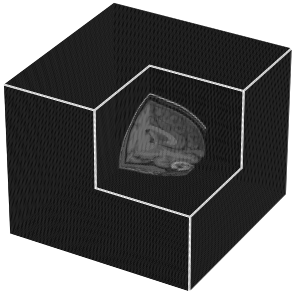
\includegraphics[height=3cm]{data/3d_bert.png}
    %             };
    %         }
    %         \visible<3-6>{
    %             \node[
    %                 font=\fontsize{10}{10}\selectfont\bfseries,
    %                 align=center,
    %                 anchor=west
    %             ] at (-4.5, 2) {
    %                 Structural Magnetic\\
    %                 Resonance Imaging (MRI) scans
    %             };

    %             \node[label=below:\small{Side}] (side) at (-3.25, -1.65) {
    %                 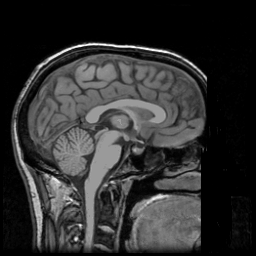
\includegraphics[height=2.5cm]{data/bert_x_enhanced.png}
    %             };

    %             \node[label=below:\small{Above}] at (0, -1.65) {
    %                 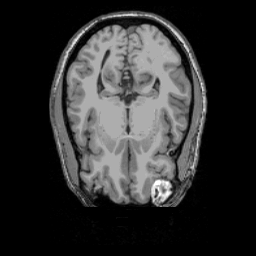
\includegraphics[height=2.5cm]{data/bert_y_enhanced.png}
    %             };

    %             \node[label=below:\small{Front}] at (3.25, -1.65) {
    %                 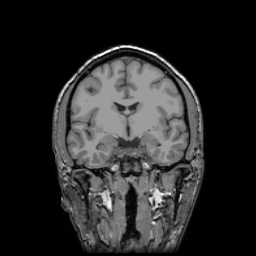
\includegraphics[height=2.5cm]{data/bert_z_enhanced.png}
    %             };
    %         }
    %         \visible<4-5>{
    %             \node[] at ($ (side.north east) + (0.5, 0.5) $) {
    %                 
\includegraphics[width=3cm]{data/region.png}
    %             };
    %             \node[
    %                 draw=red,
    %                 circle,
    %                 minimum size=3cm,
    %                 thick
    %             ] at ($ (side.north east) + (0.495, 0.495) $) {};
    %             \node[
    %                 draw=red,
    %                 circle,
    %                 minimum size=0.05cm,
    %                 inner sep=0pt,
    %             ] at ($ (side.north east) - (1.2, 1.12) $) {};
    %             \draw[red] ($ (side.north east) - (1.225, 1.12) $) --
    %                        ($ (side.north east) - (0.99, -0.75) $);
    %             \draw[red] ($ (side.north east) - (1.2, 1.145) $) --
    %                        ($ (side.north east) - (-0.75, 0.99) $);
    %         }
    %         \visible<5>{
    %             \node[
    %                 draw=red,
    %                 minimum height=0.6cm,
    %                 minimum width=0.6cm
    %             ] at ($ (side.north east) + (0.5, 0.5) $) {};

    %             \neuron{(0.1, 0.1)}{n0}
    %             \neuron{(0.05, 0.15)}{n1}
    %             \neuron{(-0.2, -0.1)}{n2}
    %             \neuron{(-0.15, 0.1)}{n3}
    %             \neuron{(0, -0.05)}{n4}
    %             \neuron{(0.13, -0.21)}{n5}
    %             \neuron{(0.15, -0.02)}{n6}
    %             \neuron{(-0.08, -0.13)}{n7}
    %             \neuron{(-0.05, 0.22)}{n8}

    %             \pgfplotsforeachungrouped  \i in {0,...,8} {
    %                 \pgfplotsforeachungrouped  \j in {0,...,8} {
    %                     \ifdim\i pt<\j pt
    %                         \draw[line width=0.25pt] (n\i) -- (n\j);
    %                     \fi
    %                 }
    %             }

    %             \neuron{(0.1, 0.1)}{n0}
    %             \neuron{(0.05, 0.15)}{n1}
    %             \neuron{(-0.2, -0.1)}{n2}
    %             \neuron{(-0.15, 0.1)}{n3}
    %             \neuron{(0, -0.05)}{n4}
    %             \neuron{(0.13, -0.21)}{n5}
    %             \neuron{(0.15, -0.02)}{n6}
    %             \neuron{(-0.08, -0.13)}{n7}
    %             \neuron{(-0.05, 0.22)}{n8}

    %         }
    %         \visible<6-7>{
    %             \node[rotate=-14, font=\small\selectfont] (label1) at ($ (threed) + (0.545, 1.46) $) {256};
    %             \node[rotate=37, font=\small\selectfont] (label2) at ($ (threed) + (-0.915, 1.3) $) {256};
    %             \node[rotate=93, font=\small\selectfont] (label3) at ($ (threed) - (1.67, 0.115) $) {256};
    %             \node[font=\boldmath] at ($ (threed.south) + (0, -0.2) $) {
    %                 $p \approx 10\,000\,000$
    %             };
    %         }
    %         \visible<7-8>{
    %             \node[] (clinical) at (-3, 0) {
    %                 \usebox{\clinical}
    %             };
    %             \node[anchor=north, align=center, font=\small\selectfont\bfseries\boldmath] at (clinical.south) {
    %                 Clinical datasets\\
    %                 ($n \approx 100$)
    %             };
    %         }
    %         \visible<8>{
    %             \node[] (population) at (3, 0) {
    %                 \usebox{\population}
    %             };
    %             \node[anchor=north, align=center, font=\small\selectfont\bfseries\boldmath] at (population.south) {
    %                 Population datasets\\
    %                 ($n \approx 10\,000$)
    %             };
    %         }
    %         \visible<9-11>{
    %             \node[anchor=west, label={[label distance=-0.15cm, anchor=north]below:\scriptsize{Generated by Dall-E 3}}] at (-5.1, 0) {
    %                 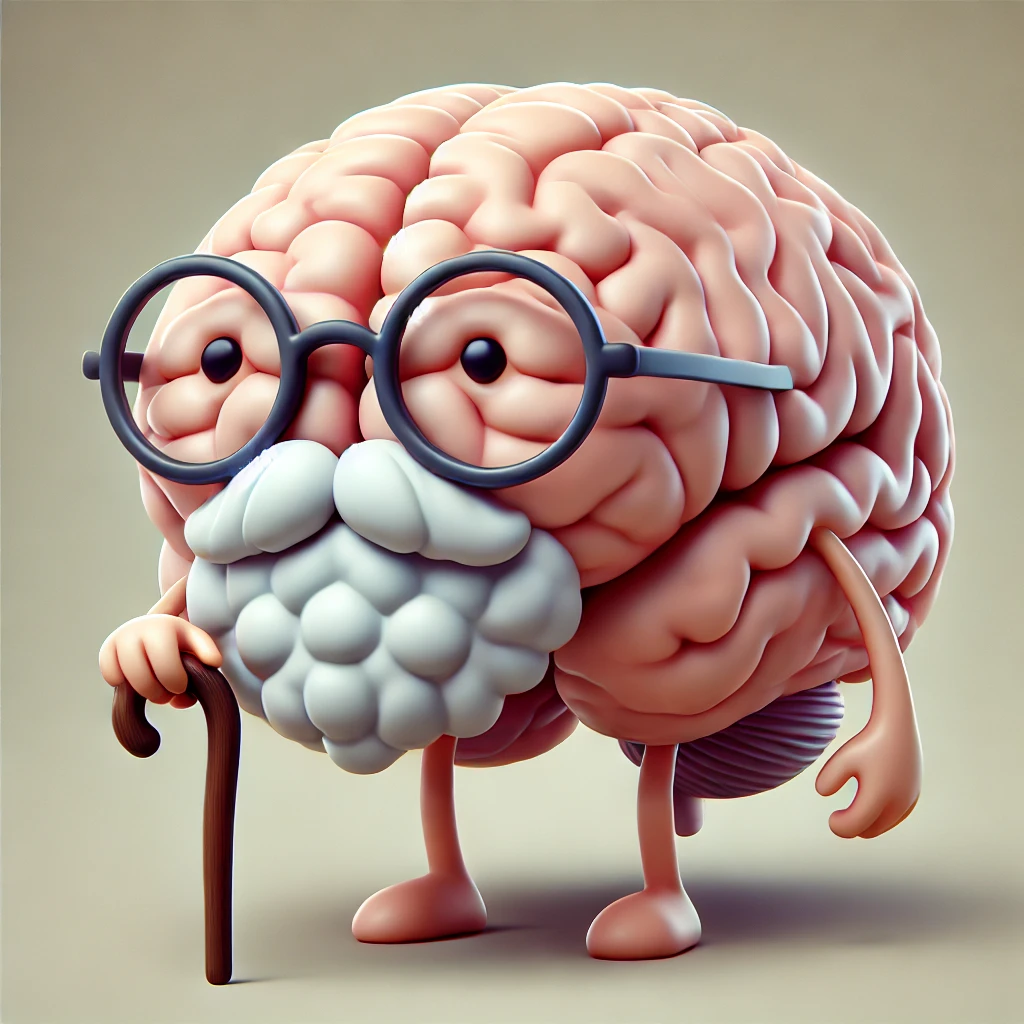
\includegraphics[width=4cm]{data/brainage.png}
    %             };
    %         }
    %         \visible<10>{
    %             \node[anchor=east] at (5.1, -0.43) {
    %                 \usebox{\brainage}
    %             };
    %         }
    %         \visible<11>{
    %             \node[anchor=east] at (5.1, -0.43) {
    %                 \usebox{\brainagepredictions}
    %             };
    %         }
    %     \end{tikzpicture}
    % \end{frame}

    % \newsavebox{\datasetbox}
    % \sbox{\datasetbox}{
    %     \begin{tikzpicture}
    %         \pgfplotstableread[col sep=comma]{data/full_data_distributions.csv}\data

    %         \begin{axis}[
    %             width=0.8\textwidth,
    %             height=0.85\textwidth,
    %             xmin=0,
    %             xmax=100,
    %             ytick=\empty,
    %             axis x line=middle,
    %             axis y line=none,
    %             xtick={10,20,30,40,50,60,70,80},
    %             x axis line style={|-stealth},
    %             clip=false
    %         ]
    %             \addplot[
    %                 name path global=zero,
    %             ] coordinates {(0,0) (100,0)};

    %             \def\previouspath{zero}

    %             \pgfplotsforeachungrouped \sex/\sign in {female/1, male/-1} {
    %                 \xdef\previouspath{zero}
    %                 % \pgfplotsforeachungrouped \dataset in {ds002424, HBN, ABCD, QTAB, PING, ADHD200, PNC, {ABIDE II}, ds000119,{ABIDE I}, BRAINMINT, SLIM, QTIM, Beijing, AOMIC-PIOP2, ds000202, AOMIC-PIOP1, CoRR, HCP, FCON1000, ds000171, TOP, SCZ-Z, NIMH, NKI-RS, MPI-LEMON, ds003592, ds004302, ds000222, SALD, IXI, DLBS, Cam-CAN, StrokeMRI, PPMI, UKBB, Tao-Wu, ds000245, OASIS3, Demgen, NEUROCON, MIRIAD, ds004392, AIBL, ANM, ADNI} {
    %                 \pgfplotsforeachungrouped \dataset in {ds002424, HBN, ABCD} {
    %                     \edef\currentpath{\sex\dataset}
    %                     \edef\currentfill{\dataset!50}
    %                     \edef\region{\previouspath\space and\space\currentpath}

    %                     \addplot [
    %                         draw=none,
    %                         line width=0pt,
    %                         name path global={\currentpath},
    %                     ] table [
    %                         x=age,
    %                         y expr=\sign * \thisrow{\sex_\dataset}
    %                     ]{\data};

    %                     \addplot[
    %                         fill=\currentfill
    %                     ] fill between [
    %                         of/.expanded={\region}
    %                     ];

    %                     \typeout{\region}
    %                 }
    %             }

    %             \node[
    %                 circle,
    %                 anchor=west,
    %                 draw=ds002424,
    %                 fill=ds002424!50,
    %                 label={[text depth=0]right:\footnotesize{ds002424}},
    %                 inner sep=2pt
    %             ] (legend1) at (axis cs: 102, 1){};
    %         \end{axis}
    %     \end{tikzpicture}
    % }

    % \newcommand{\mriinput}[2]{
    %     \def\mridepth{0.6}
    %     \node[yslant=1, inner sep=0pt] (input) at (#1, #2) {
    %         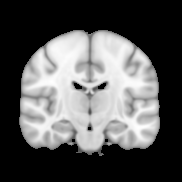
\includegraphics[height=1.7cm, width=1cm]{data/mri.png}
    %     };
    %     \draw[fill=black] (input.north east) --
    %         ($ (input.north east) - (\mridepth, 0) $) --
    %         ($ (input.north west) - (\mridepth, 0) $) --
    %         (input.north west) -- cycle;
    %     \draw[fill=black] (input.north west) --
    %         ($ (input.north west) - (\mridepth, 0) $) --
    %         ($ (input.south west) - (\mridepth, 0) $) --
    %         (input.south west) -- cycle;
    %     \draw[] (input.north east) --
    %         ($ (input.north east) + (\mridepth, 0) $) --
    %         ($ (input.north west) + (\mridepth, 0) $) --
    %         (input.north west) -- cycle;
    %     \draw[]  ($ (input.north west) + (\mridepth, 0) $) --
    %         ($ (input.south west) + (\mridepth, 0) $) --
    %         (input.south west);
    %     \draw[] ($ (input.north east) + (\mridepth, 0) $) --
    %         ($ (input.south east) + (\mridepth, 0) $) --
    %         ($ (input.south west) + (\mridepth, 0) $);
    % }

    % \newcommand{\convside}[6]{
    %     \node[
    %         fill=#5,
    %         inner sep=0pt,
    %         outer sep=0pt,
    %         minimum width=#3,
    %         minimum height=#4,
    %         draw=black
    %     ] (#6) at (#1, #2) {};
    % }

    % \newcommand{\convtop}[4]{
    %     \draw[fill=#4,draw=black] #1 --
    %     ($ #1 + (#3, #3) $) --
    %     ($ #1 + (#3+#2, #3) $) --
    %     ($ #1 + (#2, 0) $);
    % }

    % \newcommand{\convfront}[3]{
    %     \draw[black, fill=#3] #1 --
    %                         ($ #1 + (1*#2, 1*#2) $) --
    %                         ($ #1 + (1*#2, 1*#2 - 2*#2) $) --
    %                         ($ #1 + (0, -2*#2) $);
    % }


    % \newcommand{\convchannel}[5]{
    %     \def\huemin{20}
    %     \def\huemax{80}
    %     \pgfmathsetmacro{\iterations}{#5-1}
    %     \foreach \i in {0,...,\iterations} {
    %         \pgfmathsetmacro{\hue}{int(random(\huemin, \huemax))}
    %         \convside{#1}{#2+\i*-0.15}{#3}{#4/#5}{blue!\hue}{n\i0}

    %         \foreach \j in {0,...,\iterations} {
    %             \pgfmathsetmacro{\innerhue}{int(random(\huemin, \huemax))}
    %             \ifnum\j=0
    %                 \pgfmathsetmacro{\innerhue}{\hue}
    %             \fi
    %             \convfront{($ (n00.north east) + (0.5*\j*#4/#5, 0.5*\j*#4/#5 - \i*#4/#5) $)}{0.5*#4/#5}{blue!\innerhue}

    %             \ifnum\i=0
    %                 \convtop{($ (n\i0.north west) + (0.5*\j*#4/#5, 0.5*\j*#4/#5) $)}{#3}{0.5*#4/#5}{blue!\innerhue}
    %             \fi
    %         }
    %     }
    % }

    % \newcommand{\convlayer}[6]{
    %     \pgfmathsetmacro{\iterations}{#6-1}
    %     \foreach \i in {0,...,\iterations}{
    %         \pgfmathsetmacro{\x}{#1 + \i * 0.066}
    %         \convchannel{\x}{#2}{#3}{#4}{#5}
    %     }
    % }

    % \newcommand{\cnnarrow}[2]{
    %     \begin{scope}[transparency group, opacity=0.5]
    %         \draw[-stealth, line width=2pt] #1 -- #2;
    %     \end{scope}
    % }

    % \newcommand{\cnn}[2]{
    %     \convlayer{#1 - 0.06 + 0.4}{#2 + 0.38}{0.066cm}{1.8cm}{12}{3}
    %     \cnnarrow{(#1 + 0.95, #2)}{(#1+2.2, #2)}

    %     \convlayer{#1 + 1.44 + 0.4}{#2 + 0.23}{0.066cm}{1.2cm}{8}{5}
    %     \cnnarrow{(#1 + 2.43, #2)}{(#1+3.5, #2)}

    %     \convlayer{#1 + 2.77 + 0.4}{#2 + 0.08}{0.066cm}{0.6cm}{4}{7}
    %     \cnnarrow{(#1 + 3.75, #2)}{(#1+5, #2)}

    %     \convlayer{#1 + 3.93 + 0.4}{#2 + 0}{0.066cm}{0.3cm}{2}{9}

    %     \draw[thick, dashed] (#1 + 0.22, #2 + 1.43) --
    %                         (#1 + 5.13, #2 + 1.43) --
    %                         (#1 + 5.13, #2 - 1.42) --
    %                         (#1 + 0.22, #2 - 1.42) -- cycle;
    %     \node[anchor=south, text depth=0, font=\small\selectfont] at (#1 + 2.675, #2 + 1.43) {
    %         \textbf{3D Convolutional Neural Network}
    %     };
    % }

    % \newcommand{\lrpchannel}[5]{
    %     \def\huemin{30}
    %     \def\huemax{210}
    %     \colorlet{bgcolor}{black!90}
    %     \pgfmathsetmacro{\iterations}{#5-1}
    %     \foreach \i in {0,...,\iterations} {
    %         \pgfmathsetmacro{\red}{int(random(-150, 100))}
    %         \colorlet{fillcolor}{bgcolor}

    %         \ifnum\red>0
    %             \colorlet{fillcolor}{red!\red!bgcolor}
    %         \fi

    %         \convside{#1}{#2+\i*-0.75}{#3}{#4/#5}{fillcolor}{n\i0}

    %         \foreach \j in {0,...,\iterations} {
    %             \pgfmathsetmacro{\innerred}{int(random(-150, 100))}
    %             \colorlet{innerfillcolor}{bgcolor}

    %             \ifnum\innerred>0
    %                 \colorlet{innerfillcolor}{red!\innerred!bgcolor}
    %             \fi

    %             \ifnum\j=0
    %                 \colorlet{innerfillcolor}{fillcolor}
    %             \fi

    %             \convfront{($ (n00.north east) + (0.5*\j*#4/#5, 0.5*\j*#4/#5 - \i*#4/#5) $)}{0.5*#4/#5}{innerfillcolor}
    %             \ifnum\i=0
    %                 \convtop{($ (n\i0.north west) + (0.5*\j*#4/#5, 0.5*\j*#4/#5) $)}{#3}{0.5*#4/#5}{innerfillcolor}
    %             \fi
    %         }
    %     }
    % }

    % \newcommand{\lrplayer}[6]{
    %     \pgfmathsetmacro{\iterations}{#6-1}
    %     \foreach \i in {0,...,\iterations}{
    %         \pgfmathsetmacro{\x}{#1 + \i * 0.33}
    %         \lrpchannel{\x}{#2}{#3}{#4}{#5}
    %     }
    % }

    % \newcommand{\lrp}[2]{

    %     \lrplayer{#1}{#2-1}{0.33cm}{1.5cm}{2}{9}
    %     \cnnarrow{(#1 + 3.18, #2 - 1)}{(#1+6, #2 - 1)}
    %     \lrplayer{#1+4.24}{#2-0.65}{0.33cm}{3cm}{4}{7}
    %     \cnnarrow{(#1 + 7.14, #2 - 1)}{(#1+13, #2 - 1)}
    %     \lrplayer{#1 + 8.57}{#2+0.1}{0.33cm}{6cm}{8}{5}
    %     \cnnarrow{(#1 + 11.55, #2 - 1)}{(#1+15, #2 - 1)}
    %     \lrplayer{#1 + 13.72}{#2 + 0.85}{0.33cm}{9cm}{12}{3}%#1 + 14.85

    %     \draw[thick, dashed] (#1 - 0.67, #2 + 6.225) --
    %                         (#1 + 19.55, #2 + 6.225) --
    %                         (#1 + 19.55, #2 - 8.275) --
    %                         (#1 - 0.67, #2 - 8.275) -- cycle;
    %     \node[anchor=south, text depth=0, font=\fontsize{32}{32}] at (#1 + 9.95, #2 + 6.425) {
    %         \textbf{Layerwise relevance propagation}
    %     };
    % }

    % \newcommand{\heatmap}[2]{
    %     \node[yslant=1, inner sep=0pt] (map) at (#1, #2) {
    %         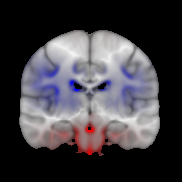
\includegraphics[width=5cm, height=8.5cm]{data/heatmap.png}
    %     };
    %     \draw[fill=black] (map.north east) --
    %         ($ (map.north east) - (\mridepth, 0) $) --
    %         ($ (map.north west) - (\mridepth, 0) $) --
    %         (map.north west) -- cycle;
    %     \draw[fill=black] (map.north west) --
    %         ($ (map.north west) - (\mridepth, 0) $) --
    %         ($ (map.south west) - (\mridepth, 0) $) --
    %         (map.south west) -- cycle;
    %     \draw[] (map.north east) --
    %         ($ (map.north east) + (\mridepth, 0) $) --
    %         ($ (map.north west) + (\mridepth, 0) $) --
    %         (map.north west) -- cycle;
    %     \draw[]  ($ (map.north west) + (\mridepth, 0) $) --
    %         ($ (map.south west) + (\mridepth, 0) $) --
    %         (map.south west);
    %     \draw[] ($ (map.north east) + (\mridepth, 0) $) --
    %         ($ (map.south east) + (\mridepth, 0) $) --
    %         ($ (map.south west) + (\mridepth, 0) $);
    %     \node[
    %         anchor=south,
    %         align=center,
    %         font=\fontsize{32}{32}\linespread{0.8}\selectfont,
    %         text depth=0
    %     ] at ($ (map.north east) + (0, 0.2) $) {
    %         \textit{Explanatory}\\
    %         \textit{heatmap}
    %     };
    % }

    % \newsavebox{\cnnforward}
    % \sbox{\cnnforward}{
    %     \begin{tikzpicture}
    %         \mriinput{-1.2}{-1.15}
    %         \cnnarrow{(input.center)}{($ (input.center) + (2, 0) $)}

    %         \cnn{0}{-1.15}

    %         \node[font=\small\linespread{0.8}\selectfont, align=center] (output) at (6.1 + 0.5, -1.15) {
    %             Chronological\\age
    %         };
    %         \cnnarrow{($ (output.west) - (0.33, 0) $)}{($ (output.west) + (0.1, 0) $)}
    %     \end{tikzpicture}
    % }

    % \newsavebox{\results}
    % \sbox{\results}{
    %     \begin{tikzpicture}
	% 		\begin{axis}[
	% 			xmin=0,
	% 			xmax=100,
	% 			ymin=0,
	% 			ymax=100,
	% 			xtick pos=bottom,
	% 			ytick pos=left,
	% 			xlabel={Chronological age},
	% 			ylabel={Predicted brain age},
    %             height=7cm,
    %             width=7cm
	% 		]
	% 			\addplot [red] coordinates {(0,0) (100,100)};
	% 			\addplot [
	% 				only marks,
	% 				mark size=2pt,
	% 				color=blue,
	% 				opacity=0.2
	% 			] table [
	% 				x=yhat,
	% 				y=y,
	% 				col sep=comma
	% 			] {data/predictions.csv};
	% 			\addplot [red] coordinates {(0,0) (100,100)};
	% 			\node [anchor=south east,inner sep=0pt,outer sep=0pt] (outofsample) at (rel axis cs:0.92,0.08) {\textcolor{red}{MAE=4.73}};
	% 		\end{axis}
	% 	\end{tikzpicture}
    % }

    \newcommand{\disorderplot}[3]{
        \nextgroupplot[
            xticklabels={#2},
            xlabel={#3}
        ]
            \addplot [
                draw=none,
                line width=0pt,
                name path=zero,
            ] coordinates {(0,0) (15,0)};

            \addplot [
                draw=none,
                line width=0pt,
                name path=#1-HC,
            ] table [
                col sep=comma,
                x=x,
                y=#1-HC
            ] {data/disorders.csv};

            \addplot[
                HC,
                opacity=0.75,
            ] fill between [
                of=zero and #1-HC
            ];

            \addplot [
                draw=none,
                line width=0pt,
                name path=#1,
            ] table [
                col sep=comma,
                x=x,
                y=#1
            ] {data/disorders.csv};

            \addplot[
                #1,
                opacity=0.75,
            ] fill between [
                of=zero and #1
            ];
    }

    \newsavebox{\patients}
    \sbox{\patients}{
        \newcommand{\legendnode}[4]{
            \node[align=left, font=\tiny\selectfont, anchor=west] at #1 {
                \textbf{#2}\\
                $\Delta$=#3 (p=$#4$)
            };
        }
        \begin{tikzpicture}
            \begin{groupplot}[
                group style={
                    group size=1 by 9,
                    vertical sep=0.05cm,
                    group name=group
                },
                height=2.23cm,
                width=9cm,
                xmin=-15,
                xmax=15,
                ymax=1,
                ymin=0,
                ytick=\empty,
                axis x line=bottom,
                xtick={-10,0,10},
                xticklabels=\empty,
                axis y line=none,
                x axis line style={stealth-stealth},
                clip=false,
                xticklabel style={font=\footnotesize},
                xlabel style={font=\footnotesize, yshift=0.15cm},
            ]
                \disorderplot{DEM}{\empty}{}
                \disorderplot{MS}{\empty}{}
                \disorderplot{MCI}{\empty}{}
                \disorderplot{SCZ}{\empty}{}
                \disorderplot{ANX}{\empty}{}
                \disorderplot{BIP}{\empty}{}
                \disorderplot{ASD}{\empty}{}
                \disorderplot{MDD}{\empty}{}
                \disorderplot{ADHD}{{-10,0,10}}{Brain age delta}

            \end{groupplot}
            \legendnode{($ (group c1r1.west) + (0, 0) $)}{Dementia}{5.10}{2.53\times10^{-48}}
            \legendnode{($ (group c1r2.west) + (0, 0) $)}{Multiple sclerosis}{3.82}{1.35\times10^{-9}}
            \legendnode{($ (group c1r3.west) + (0, 0) $)}{Mild cognitive impairment}{1.75}{7.64\times10^{-8}}
            \legendnode{($ (group c1r4.west) + (0, 0) $)}{Schizophrenia}{1.26}{4.34\times10^{-4}}
            \legendnode{($ (group c1r5.west) + (0, 0) $)}{Anxiety disorders}{1.00}{0.17}
            \legendnode{($ (group c1r6.west) + (0, 0) $)}{Bipolar disorder}{0.86}{0.04}
            \legendnode{($ (group c1r7.west) + (0, 0) $)}{Autism spectrum disorder}{0.38}{0.20}
            \legendnode{($ (group c1r8.west) + (0, 0) $)}{Major depressive disorder}{0.08}{0.93}
            \legendnode{($ (group c1r9.west) + (0, 0) $)}{Attention deficit/hyperactivity disorder}{-0.07}{0.81}
        \end{tikzpicture}
    }

    \newsavebox{\dementiapatients}
    \sbox{\dementiapatients}{
        \begin{tikzpicture}
            \begin{axis}[
                height=5cm,
                width=9cm,
                xmin=-15,
                xmax=15,
                ymax=1,
                ymin=0,
                ytick=\empty,
                axis x line=bottom,
                xtick={-10,0,10},
                axis y line=none,
                x axis line style={stealth-stealth},
                clip=false,
                xticklabel style={font=\footnotesize},
                xlabel style={font=\footnotesize, yshift=0.15cm},
                xlabel={Brain age delta}
            ]
                \addplot [
                    draw=none,
                    line width=0pt,
                    name path=zero,
                ] coordinates {(0,0) (15,0)};

                \addplot [
                    draw=none,
                    line width=0pt,
                    name path=DEM-HC,
                ] table [
                    col sep=comma,
                    x=x,
                    y=DEM-HC
                ] {data/disorders.csv};

                \addplot[
                    HC,
                    opacity=0.75,
                ] fill between [
                    of=zero and DEM-HC
                ];

                \addplot [
                    draw=none,
                    line width=0pt,
                    name path=DEM,
                ] table [
                    col sep=comma,
                    x=x,
                    y=DEM
                ] {data/disorders.csv};

                \addplot[
                    DEM,
                    opacity=0.75,
                ] fill between [
                    of=zero and DEM
                ];
            \end{axis}
        \end{tikzpicture}
    }

    \begin{frame}{Brain age modelling}
        \begin{tikzpicture}
            \node[draw=black] at (-5.25, -3.5) {};
            \node[draw=black] at (5.25, 3.5) {};

            % \visible<1>{
            %     \node[] at (0, 0) {
            %         \usebox{\datasetbox}
            %     };
            % }

            % \visible<2>{
            %     \node[] at (0, 0) {
            %         \usebox{\cnnforward}
            %     };
            % }

            % \visible<3>{
            %     \node[] at (0, 0) {
            %         \usebox{\results}
            %     };
            % }

            \visible<4>{
                \node[] at (0, 0) {
                    \usebox{\patients}
                };
            }

            \visible<5>{
                \node[] at (0, 0) {
                    \usebox{\dementiapatients}
                };
            }
        \end{tikzpicture}
    \end{frame}

\end{document}
